
\documentclass[10pt]{article}

   \addtolength{\oddsidemargin} {-0.9in}
   \addtolength{\textwidth}{1.7in}
   \addtolength{\topmargin}{-1.2in}
   \addtolength{\textheight}{2in}
   \linespread{1.1}
   \usepackage{graphicx}
   \usepackage{subfig}
   \usepackage{fancyhdr}
   \usepackage{url}
   \usepackage{amsmath,amssymb}
   \usepackage{comment}
   \usepackage{float}
   \pagestyle{fancy}
\lhead{} \chead{} \rhead{} \cfoot{} \rfoot{\thepage}
\renewcommand{\headrulewidth}{0.0pt}
\renewcommand{\footrulewidth}{0.4pt}
\usepackage{xcolor}
\definecolor{mygray}{gray}{0.9}
\usepackage[colorlinks=true,linkcolor=blue,citecolor=blue,urlcolor=blue]{hyperref}
\usepackage{chemmacros}

\usepackage{listings}
\usepackage{color} %red, green, blue, yellow, cyan, magenta, black, white
\definecolor{mygreen}{RGB}{28,172,0} % color values Red, Green, Blue
\definecolor{mylilas}{RGB}{170,55,241}

\lstset{language=Matlab,%
    breaklines=true,%
    morekeywords={matlab2tikz},
    keywordstyle=\color{blue},%
    morekeywords=[2]{1}, keywordstyle=[2]{\color{black}},
    identifierstyle=\color{black},%
    stringstyle=\color{mylilas},
    commentstyle=\color{mygreen},%
    showstringspaces=false,%without this there will be a symbol in the places where there is a space
    numbers=left,%
    numberstyle={\tiny \color{black}},% size of the numbers
    numbersep=9pt, % this defines how far the numbers are from the text
    emph=[1]{for,end,break},emphstyle=[1]\color{red}, %some words to emphasise
}

\begin{document}

\begin{center}
{\Large\bf Homework \#9}\\
 {\bf Name: Andrea Livingston}\\
 {\bf Due: December 5th, 2016}\\
 {\bf CBE660: Intermediate Problems in Chemical and Biological
Engineering\; -\; Fall 2016}\\
Department of Chemical and Biological Engineering, University of Wisconsin-Madison
\end{center}

\noindent\colorbox{mygray}{\begin{minipage}{\textwidth}
  {\bf Problem 1}. Solve Exercise 4.15 in the textbook and reproduce Figures 4.2 and 4.3 in page 360.
\end{minipage}}
\\

{\em Solution:}   
\\
\\
Rearranging $x^TAx=b$ gives $f(x)=x^TAx-b$. To find the side length, c, we must minimize $f(x)$ s.t. $c=e_i^Tx$ where $e_i$ is the $i^{th}$ column (or row) of the identity matrix. 
\[ f(x)=x^TAx-b \]
Define the Lagrange problem 
\[ L=x^TAx-\lambda(e_i^Tx-c) \]
At the minimum $\frac{d L}{dx}=0$ and $\frac{d L}{d \lambda}=0$

\[ \frac{d L}{dx}=0=Ax+A^Tx-\lambda e_i = 2Ax-\lambda e_i \]
\[ \frac{d L}{d \lambda}=0=e_i^Tx-c=0 \]
\[ \begin{bmatrix} 2a & -e_i \\ e_i & 0 \end{bmatrix} \begin{bmatrix} x \\ \lambda \end{bmatrix} = \begin{bmatrix} 0 \\ -c \end{bmatrix} \]
Solve $\frac{d L}{dx}$ for x. 

\[ 2Ax=\lambda e_i \]
\[ x=\frac{1}{2}A^{-1}e_i \lambda \]
Substitute x into $\frac{d L}{d \lambda}$ and solve for $\lambda$

\[ e_i^T x=c \]
\[ e_i^T\left( \frac{1}{2}A^{-1}e_i \lambda \right)=c \]
\[ \lambda = \frac{2c}{e_i^T A^{-1}e_i} \]
Let $e_i^T A^{-1}e_i={\widetilde A}_{ii}$
\[\lambda=\frac{2c}{{\widetilde A}_{ii}} \]
Substitute the expression for $\lambda$ into $x$
\[ x=\frac{1}{2}A^{-1}e_i \lambda \]
\[ x=\frac{1}{2}A^{-1}e_i \frac{2c}{{\widetilde A}_{ii}} \]
\[ x=A^{-1}e_i \frac{c}{{\widetilde A}_{ii}} \]
substitute $x$ into the original expression $x^TAx=b$ and solve for $c$
\[ b=x^TAx \]
\[ b = \frac{c}{{\widetilde A}_{ii}} e_i^T A^{-1} A A^{-1}e_i \frac{c}{{\widetilde A}_{ii}} \]
\[ b = \left(\frac{c}{{\widetilde A}_{ii}}\right)^2 e_i^TA^{-1}e_i  = \left(\frac{c}{{\widetilde A}_{ii}}\right)^2 {\widetilde A}_{ii} = \frac{c^2}{{\widetilde A}_{ii}} \]
\[ c=\sqrt{b {\widetilde A}_{ii}} \]

\noindent
Figure 4.2 was recreated by creating a 2-dimensional normal probability distribution with an expected value of zero for both $x1$ and $x2$. The Matlab function "Contour" was used to create 'slices' of the probability distribution at given values. Figure 4.3 was recreated by taking one of those 'slices', given by a representative matrix $A$ and applying the results to show the minimum rectangle and the radii. 
\begin{figure} [H]
\subfloat[ ]{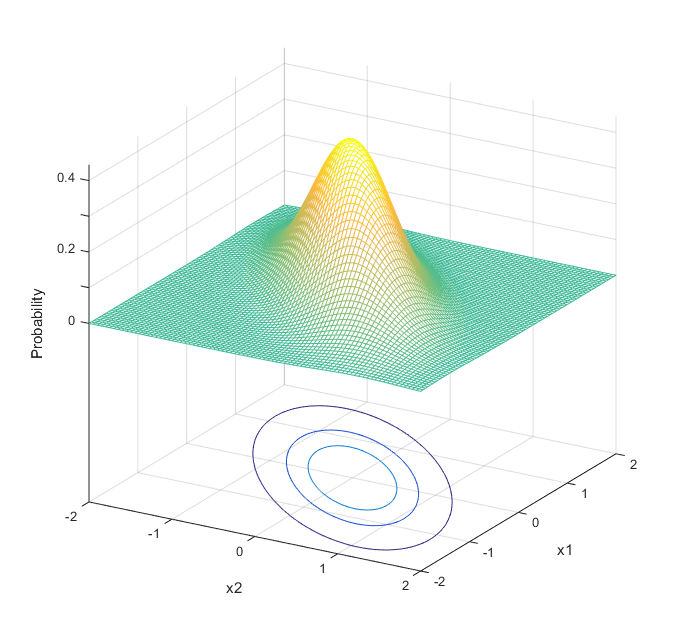
\includegraphics [width=2.5in] {CBE660_Assign9__1a.png}}
\subfloat[ ]{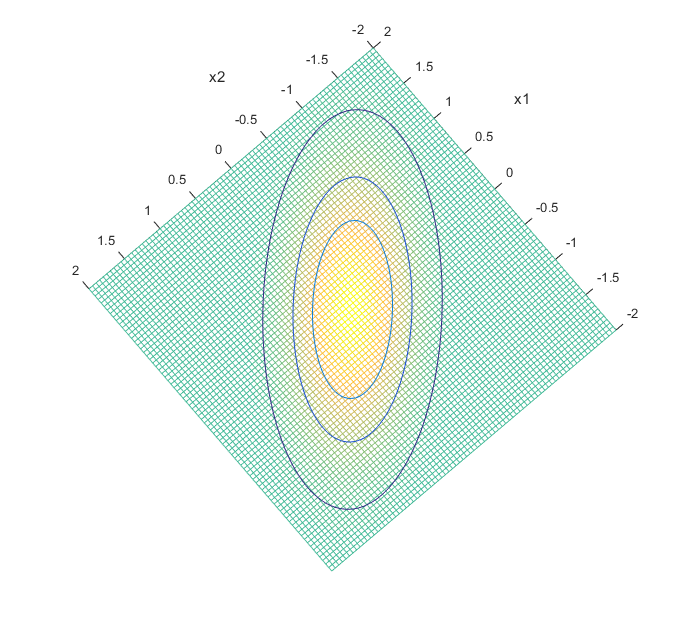
\includegraphics [width=2.5in] {CBE660_Assign9__1b.png}}
\subfloat[ ]{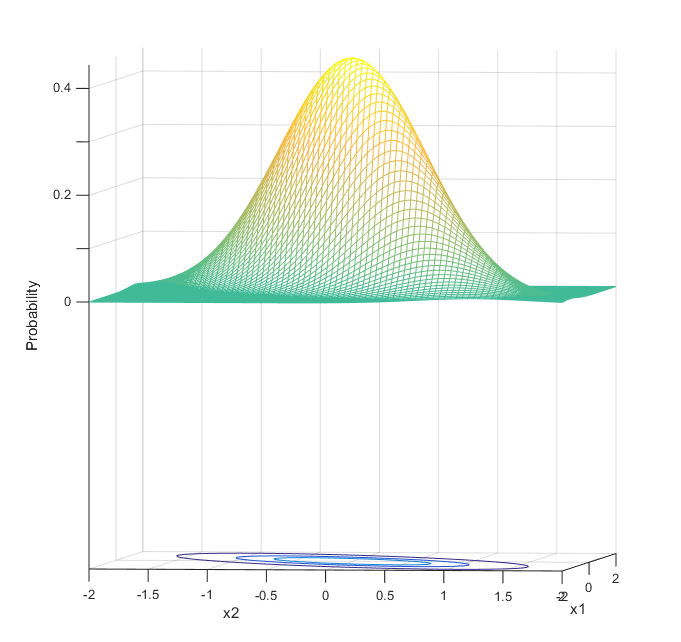
\includegraphics [width=2.5in] {CBE660_Assign9__1c.png}}
\end{figure}

{\centering
\begin{figure} [H]
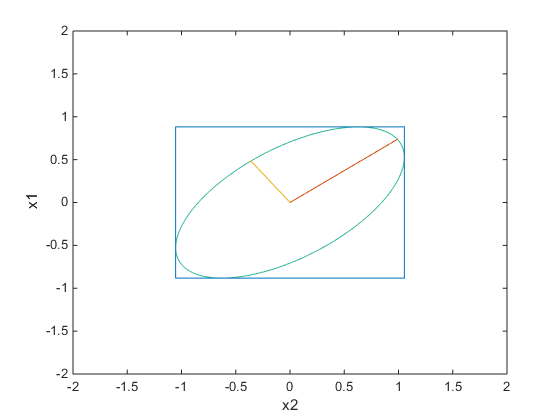
\includegraphics  {CBE660_Assign9__1d.png}
\end{figure} }

\lstinputlisting{CBE660_Assign9_1a.m}


\newpage

\noindent\colorbox{mygray}{\begin{minipage}{\textwidth}
  {\bf Problem 2}. Solve Exercise 4.1 in the textbook.
  \end{minipage}}
\\

{\em Solution:}   
\\
\\
{\bf 2.a} \\
If B contains some or all of the elements of A (\( B \subseteq A \)), what is the probability that a given element from set A is not in set B? \\
\[ Pr(x:x \in A \;and\; x\not\in B) = Pr(A)-Pr(B) \]
Define $C=A\setminus B$
\[ Pr(B \cup C)= Pr(B)+Pr(C)-Pr(B \cap C) \]
Where the \( Pr(B \cap C)=0 \) by definition of $C$, because we know that $C$ only contains elements that are not in $B$. Therefore, it is impossible for an element to belong to both $B$ and $C$. 
\[ Pr(B \cup C)=Pr(B)+Pr(C) \]
We know that $ Pr(B \cup C)=Pr(A)$
\[ Pr(B \cup C)=Pr(A)=Pr(B)+Pr(C)=Pr(B)+Pr(A\setminus B) \]
\[ Pr(A)=Pr(B)+Pr(A\setminus B) \]
\[ Pr(A\setminus B)=Pr(A)-Pr(B) \]
\\
\\
{\bf 2.b}
\\
\[ Pr(A\cap B)=Pr(A)Pr(B) \]
Using
\[ Pr(A \cup {\bar A}=Pr(A)+Pr(\bar{A})=1 \]
\[ Pr(A \cup B) = Pr(A)+Pr(B) \]
We can see that
\[ Pr(A \cap B) = (1-Pr({\bar A}))(1-Pr({\bar B})) \]
\[ Pr(A \cap B) = 1 - Pr(\bar{A})-Pr(\bar{B})+Pr(\bar{A})Pr(\bar{B}) \]
\[ Pr(A \cap B) - 1 +  Pr(\bar{A}) + Pr(\bar{B})=Pr(\bar{A})Pr(\bar{B}) \]
\[ 1-Pr(A \cap B) -\left[ Pr(\bar{A}) + Pr(\bar{B}) \right] =-Pr(\bar{A})Pr(\bar{B}) \]
Using the consequence
\[ Pr(\bar{A}) + Pr(\bar{B} = Pr(\bar{A} \cup \bar{B}) +Pr(\bar{A} \cap \bar{B})  \]
We can say that
\[ 1-Pr(A \cap B) - Pr(\bar{A} \cup \bar{B}) -Pr(\bar{A} \cap \bar{B}) =-Pr(\bar{A})Pr(\bar{B}) \]
$Pr(\bar{A} \cup \bar{B})$ is everything except $Pr(A\cap B)$. Therefore, by inspection, we can say that $Pr(A\cap B) + Pr(\bar{A} \cup \bar{B}) = 1$. Note the mistake in the figure where green should be $Pr(\bar{A} \cap \bar{B})$.

\begin{figure} [H]
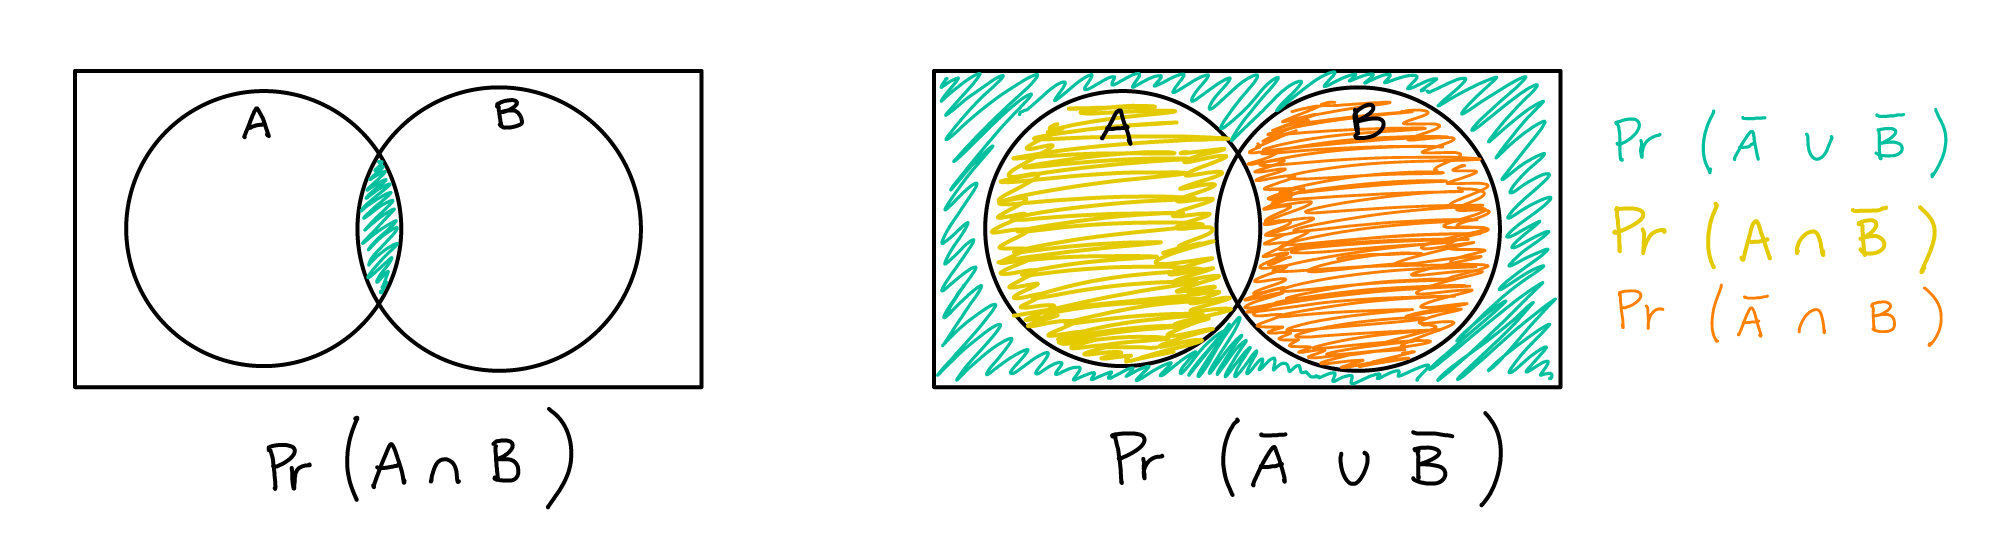
\includegraphics [width=6in] {CBE660_HW9_3.png}
\end{figure}

\[ 1-1-Pr(\bar{A} \cap \bar{B}) =-Pr(\bar{A})Pr(\bar{B}) \]
\[ Pr(\bar{A} \cap \bar{B}) =Pr(\bar{A})Pr(\bar{B}) \]
\\
Thus if $A$ and $B$ are independent $\bar{A}$ and $\bar{B}$ will also be independent. 



\newpage

\noindent\colorbox{mygray}{\begin{minipage}{\textwidth}
  {\bf Problem 3}.  Solve Exercise 4.2 in the textbook.\\ Show that \( \xi\) and \( \eta\) are statistically independent if and only if 
\[ p_{\xi,\eta}(x,y)=p_{\xi}(x)p_{\eta}(y) \]
\end{minipage}}
\\

{\em Solution:}   
\\
\\
Beginning with the probability function, assume that it can be separated into $P_{\xi,\eta}=P_\xi(x)P_eta(y)$. Integrating both sides with respect to x and y yields
\[ \int_{-\infty}^y \int_{-\infty}^x P_{\xi,\eta} dx dy = \int_{-\infty}^y \int_{-\infty}^x P_\xi(x)P_\eta(y)dxdy \]
The integrals can then be separated because $P_\xi(x)$ does not depend on y and $P_\eta(y)$ does not depend on x. 
\[ \int_{-\infty}^y \int_{-\infty}^x P_{\xi,\eta} dx dy = \int_{-\infty}^x P_\xi(x)dx \int_{-\infty}^y P_\eta(y)dy \]
Using equation 4.1 to relate the cumulative probability distribution function (CDF) to the probability density function (PDF) yields equation 4.25 for independent random variables. 
\[ \int_{-\infty}^y \int_{-\infty}^x P_{\xi,\eta} dx dy = F_\xi(x) F_\eta(y) \]
\[ F_{\xi,\eta}(x,y)= F_\xi(x) F_\eta(y)\]
\\
Thus, if the original statement for the probability density function holds, then $\xi$ and $\eta$ must be statistically independent. \\
\\
From equation 4.25 for independent random variables

\[ F_{\xi,\eta}(x,y)= F_\xi(x) F_\eta(y) \]
Again using equation 4.1 to relate the CDF's to PFD's
\[  F_{\xi,\eta}(x,y) = \int_{-\infty}^x P_\xi(x)dx \int_{-\infty}^y P_\eta(y)dy \]
\[ F_{\xi,\eta}(x,y) = \int_{-\infty}^y \int_{-\infty}^x  P_\xi(x)  P_\eta(y)dxdy \]
The relationship only holds for all x and y when the integrands are equal.
\[ \int_{-\infty}^x \int_{-\infty}^y P_\xi(x)  P_\eta(y) dx dy =  \int_{-\infty}^y \int_{-\infty}^x P_{\xi,\eta} dx dy \]
\[ \int_{-\infty}^x \int_{-\infty}^y \left( P_{\xi,\eta}(x,y)- P_\xi(x)  P_\eta(y)\right) dx dy =0 \]
\[ P_{\xi,\eta}(x,y)- P_\xi(x)  P_\eta(y) =0 \]
\\
Thus, $\xi$ and $\eta$ are statistically independent if and only if the original PDF separation is true.  





\newpage

\noindent\colorbox{mygray}{\begin{minipage}{\textwidth}
  {\bf Problem 4}.  Consider random variable $X\sim \mathcal{N}(\mu,\sigma^2)$ and constants $a,b\in\mathbb{R}$. Use the characteristic function to prove that the random variable $Y=a+bX$ is also normally distributed and find its mean and variance. 
\end{minipage}}
\\

{\em Solution:}  
\\
The Characteristic Function for normal density is
\[ \varphi_{\xi}(t)=E[e^{it\xi}]=\int_{-\infty}^{\infty}e^{itx}p_\xi(x)dX = exp[it\mu-\frac{1}{2}t^2\sigma^2] \]
\\
The characteristic equation for $Y$ then becomes
\[\varphi_Y(t)=E[e^{itY}]=E[e^{it(a+bX)}]=E[e^{ita}e^{itbX}] \]
\[\varphi_Y(t)=\int_{-\infty}^{\infty}e^{ita}e^{itbX}p_X(bX)dX \]
\[\varphi_Y(t)=e^{ita}\int_{-\infty}^{\infty}e^{itbX}p_X(bX)dX \]
Using the transformation into the t-domain from example 4.1 where now t is multiplied by the constant b
\[ \varphi_Y(t)=e^{ita}exp[itb\mu_X-\frac{1}{2}(bt)^2\sigma_X^2] \]
\[ \varphi_Y(t)=e^{ita}exp[itb\mu_X-\frac{1}{2}b^2t^2\sigma_X^2] \]

\noindent
Using the property for multiplication by a constant (equation 4.7) where $\eta=a \xi $
\[ \varphi_{\eta}(t)=\varphi_{\xi}(at) \]
And the property for addition (equation 4.8) where $\eta=\xi_1+\xi_2$
\[\varphi_\eta(t)=\varphi_{\xi_1}(t)\varphi_{\xi_2}(t) \]
We can conclude that 
\[ \varphi_Y(t)=\varphi_a(t)\varphi_{X}(bt)= e^{ita}exp[itb\mu_X-\frac{1}{2}b^2t^2\sigma_X^2]\]
\\
By inspection we can see that $\varphi_a(t)=e^{ita}$ and $\varphi_{X}(bt)=exp[itb\mu_X-\frac{1}{2}b^2t^2\sigma_X^2]$. Because the expression for $\varphi_Y(t)$ can be separated into the form given by a normal distribution, we can conclude that Y has a normal distribution. 

\[ \varphi_Y(t)=exp[itb\mu_X+ita-\frac{1}{2}b^2t^2\sigma_X^2] \]
\[ \varphi_Y(t)=exp[it(b\mu_X+a)-\frac{1}{2}b^2t^2\sigma_X^2] \]
\\
From this expression, the mean becomes $\mu_Y=b\mu_X-a$ and the variance becomes $b^2\sigma_X^2$. ;
\[ E_Y[b\mu_X-a] \]
\[ Var(Y)=b^2\sigma_X^2 \]

\end{document}


